\documentclass{ximera}

%\usepackage{todonotes}

\newcommand{\todo}{}

\usepackage{esint} % for \oiint
\ifxake%%https://math.meta.stackexchange.com/questions/9973/how-do-you-render-a-closed-surface-double-integral
\renewcommand{\oiint}{{\large\bigcirc}\kern-1.56em\iint}
\fi


\graphicspath{
  {./}
  {ximeraTutorial/}
  {basicPhilosophy/}
  {functionsOfSeveralVariables/}
  {normalVectors/}
  {lagrangeMultipliers/}
  {vectorFields/}
  {greensTheorem/}
  {shapeOfThingsToCome/}
  {dotProducts/}
  {partialDerivativesAndTheGradientVector/}
  {../productAndQuotientRules/exercises/}
  {../normalVectors/exercisesParametricPlots/}
  {../continuityOfFunctionsOfSeveralVariables/exercises/}
  {../partialDerivativesAndTheGradientVector/exercises/}
  {../directionalDerivativeAndChainRule/exercises/}
  {../commonCoordinates/exercisesCylindricalCoordinates/}
  {../commonCoordinates/exercisesSphericalCoordinates/}
  {../greensTheorem/exercisesCurlAndLineIntegrals/}
  {../greensTheorem/exercisesDivergenceAndLineIntegrals/}
  {../shapeOfThingsToCome/exercisesDivergenceTheorem/}
  {../greensTheorem/}
  {../shapeOfThingsToCome/}
  {../separableDifferentialEquations/exercises/}
  {vectorFields/}
}

\newcommand{\mooculus}{\textsf{\textbf{MOOC}\textnormal{\textsf{ULUS}}}}

\usepackage{tkz-euclide}
\usepackage{tikz}
\usepackage{tikz-cd}
\usetikzlibrary{arrows}
\tikzset{>=stealth,commutative diagrams/.cd,
  arrow style=tikz,diagrams={>=stealth}} %% cool arrow head
\tikzset{shorten <>/.style={ shorten >=#1, shorten <=#1 } } %% allows shorter vectors

\usetikzlibrary{backgrounds} %% for boxes around graphs
\usetikzlibrary{shapes,positioning}  %% Clouds and stars
\usetikzlibrary{matrix} %% for matrix
\usepgfplotslibrary{polar} %% for polar plots
\usepgfplotslibrary{fillbetween} %% to shade area between curves in TikZ
%\usetkzobj{all}
\usepackage[makeroom]{cancel} %% for strike outs
%\usepackage{mathtools} %% for pretty underbrace % Breaks Ximera
%\usepackage{multicol}
\usepackage{pgffor} %% required for integral for loops



%% http://tex.stackexchange.com/questions/66490/drawing-a-tikz-arc-specifying-the-center
%% Draws beach ball
\tikzset{pics/carc/.style args={#1:#2:#3}{code={\draw[pic actions] (#1:#3) arc(#1:#2:#3);}}}



\usepackage{array}
\setlength{\extrarowheight}{+.1cm}
\newdimen\digitwidth
\settowidth\digitwidth{9}
\def\divrule#1#2{
\noalign{\moveright#1\digitwidth
\vbox{\hrule width#2\digitwidth}}}




% \newcommand{\RR}{\mathbb R}
% \newcommand{\R}{\mathbb R}
% \newcommand{\N}{\mathbb N}
% \newcommand{\Z}{\mathbb Z}

\newcommand{\sagemath}{\textsf{SageMath}}


%\renewcommand{\d}{\,d\!}
%\renewcommand{\d}{\mathop{}\!d}
%\newcommand{\dd}[2][]{\frac{\d #1}{\d #2}}
%\newcommand{\pp}[2][]{\frac{\partial #1}{\partial #2}}
% \renewcommand{\l}{\ell}
%\newcommand{\ddx}{\frac{d}{\d x}}

% \newcommand{\zeroOverZero}{\ensuremath{\boldsymbol{\tfrac{0}{0}}}}
%\newcommand{\inftyOverInfty}{\ensuremath{\boldsymbol{\tfrac{\infty}{\infty}}}}
%\newcommand{\zeroOverInfty}{\ensuremath{\boldsymbol{\tfrac{0}{\infty}}}}
%\newcommand{\zeroTimesInfty}{\ensuremath{\small\boldsymbol{0\cdot \infty}}}
%\newcommand{\inftyMinusInfty}{\ensuremath{\small\boldsymbol{\infty - \infty}}}
%\newcommand{\oneToInfty}{\ensuremath{\boldsymbol{1^\infty}}}
%\newcommand{\zeroToZero}{\ensuremath{\boldsymbol{0^0}}}
%\newcommand{\inftyToZero}{\ensuremath{\boldsymbol{\infty^0}}}



% \newcommand{\numOverZero}{\ensuremath{\boldsymbol{\tfrac{\#}{0}}}}
% \newcommand{\dfn}{\textbf}
% \newcommand{\unit}{\,\mathrm}
% \newcommand{\unit}{\mathop{}\!\mathrm}
% \newcommand{\eval}[1]{\bigg[ #1 \bigg]}
% \newcommand{\seq}[1]{\left( #1 \right)}
% \renewcommand{\epsilon}{\varepsilon}
% \renewcommand{\phi}{\varphi}


% \renewcommand{\iff}{\Leftrightarrow}

% \DeclareMathOperator{\arccot}{arccot}
% \DeclareMathOperator{\arcsec}{arcsec}
% \DeclareMathOperator{\arccsc}{arccsc}
% \DeclareMathOperator{\si}{Si}
% \DeclareMathOperator{\scal}{scal}
% \DeclareMathOperator{\sign}{sign}


%% \newcommand{\tightoverset}[2]{% for arrow vec
%%   \mathop{#2}\limits^{\vbox to -.5ex{\kern-0.75ex\hbox{$#1$}\vss}}}
% \newcommand{\arrowvec}[1]{{\overset{\rightharpoonup}{#1}}}
% \renewcommand{\vec}[1]{\arrowvec{\mathbf{#1}}}
% \renewcommand{\vec}[1]{{\overset{\boldsymbol{\rightharpoonup}}{\mathbf{#1}}}}

% \newcommand{\point}[1]{\left(#1\right)} %this allows \vector{ to be changed to \vector{ with a quick find and replace
% \newcommand{\pt}[1]{\mathbf{#1}} %this allows \vec{ to be changed to \vec{ with a quick find and replace
% \newcommand{\Lim}[2]{\lim_{\point{#1} \to \point{#2}}} %Bart, I changed this to point since I want to use it.  It runs through both of the exercise and exerciseE files in limits section, which is why it was in each document to start with.

% \DeclareMathOperator{\proj}{\mathbf{proj}}
% \newcommand{\veci}{{\boldsymbol{\hat{\imath}}}}
% \newcommand{\vecj}{{\boldsymbol{\hat{\jmath}}}}
% \newcommand{\veck}{{\boldsymbol{\hat{k}}}}
% \newcommand{\vecl}{\vec{\boldsymbol{\l}}}
% \newcommand{\uvec}[1]{\mathbf{\hat{#1}}}
% \newcommand{\utan}{\mathbf{\hat{t}}}
% \newcommand{\unormal}{\mathbf{\hat{n}}}
% \newcommand{\ubinormal}{\mathbf{\hat{b}}}

% \newcommand{\dotp}{\bullet}
% \newcommand{\cross}{\boldsymbol\times}
% \newcommand{\grad}{\boldsymbol\nabla}
% \newcommand{\divergence}{\grad\dotp}
% \newcommand{\curl}{\grad\cross}
%\DeclareMathOperator{\divergence}{divergence}
%\DeclareMathOperator{\curl}[1]{\grad\cross #1}
% \newcommand{\lto}{\mathop{\longrightarrow\,}\limits}

% \renewcommand{\bar}{\overline}

\colorlet{textColor}{black}
\colorlet{background}{white}
\colorlet{penColor}{blue!50!black} % Color of a curve in a plot
\colorlet{penColor2}{red!50!black}% Color of a curve in a plot
\colorlet{penColor3}{red!50!blue} % Color of a curve in a plot
\colorlet{penColor4}{green!50!black} % Color of a curve in a plot
\colorlet{penColor5}{orange!80!black} % Color of a curve in a plot
\colorlet{penColor6}{yellow!70!black} % Color of a curve in a plot
\colorlet{fill1}{penColor!20} % Color of fill in a plot
\colorlet{fill2}{penColor2!20} % Color of fill in a plot
\colorlet{fillp}{fill1} % Color of positive area
\colorlet{filln}{penColor2!20} % Color of negative area
\colorlet{fill3}{penColor3!20} % Fill
\colorlet{fill4}{penColor4!20} % Fill
\colorlet{fill5}{penColor5!20} % Fill
\colorlet{gridColor}{gray!50} % Color of grid in a plot

\newcommand{\surfaceColor}{violet}
\newcommand{\surfaceColorTwo}{redyellow}
\newcommand{\sliceColor}{greenyellow}




\pgfmathdeclarefunction{gauss}{2}{% gives gaussian
  \pgfmathparse{1/(#2*sqrt(2*pi))*exp(-((x-#1)^2)/(2*#2^2))}%
}


%%%%%%%%%%%%%
%% Vectors
%%%%%%%%%%%%%

%% Simple horiz vectors
\renewcommand{\vector}[1]{\left\langle #1\right\rangle}


%% %% Complex Horiz Vectors with angle brackets
%% \makeatletter
%% \renewcommand{\vector}[2][ , ]{\left\langle%
%%   \def\nextitem{\def\nextitem{#1}}%
%%   \@for \el:=#2\do{\nextitem\el}\right\rangle%
%% }
%% \makeatother

%% %% Vertical Vectors
%% \def\vector#1{\begin{bmatrix}\vecListA#1,,\end{bmatrix}}
%% \def\vecListA#1,{\if,#1,\else #1\cr \expandafter \vecListA \fi}

%%%%%%%%%%%%%
%% End of vectors
%%%%%%%%%%%%%

%\newcommand{\fullwidth}{}
%\newcommand{\normalwidth}{}



%% makes a snazzy t-chart for evaluating functions
%\newenvironment{tchart}{\rowcolors{2}{}{background!90!textColor}\array}{\endarray}

%%This is to help with formatting on future title pages.
\newenvironment{sectionOutcomes}{}{}



%% Flowchart stuff
%\tikzstyle{startstop} = [rectangle, rounded corners, minimum width=3cm, minimum height=1cm,text centered, draw=black]
%\tikzstyle{question} = [rectangle, minimum width=3cm, minimum height=1cm, text centered, draw=black]
%\tikzstyle{decision} = [trapezium, trapezium left angle=70, trapezium right angle=110, minimum width=3cm, minimum height=1cm, text centered, draw=black]
%\tikzstyle{question} = [rectangle, rounded corners, minimum width=3cm, minimum height=1cm,text centered, draw=black]
%\tikzstyle{process} = [rectangle, minimum width=3cm, minimum height=1cm, text centered, draw=black]
%\tikzstyle{decision} = [trapezium, trapezium left angle=70, trapezium right angle=110, minimum width=3cm, minimum height=1cm, text centered, draw=black]


\title{Notation}

\begin{document}

\begin{abstract}
$a + b \, i$
\end{abstract}
\maketitle


So, far our 2-dimensional arithmetic has a strong geometric flavor.  In this section, we will introduce a new layer of abbreviations and notation, that will give our new arithmetic a more algebraic feel. 


We are currently representing our new numbers with 2-dimensional vectors.

\begin{image}
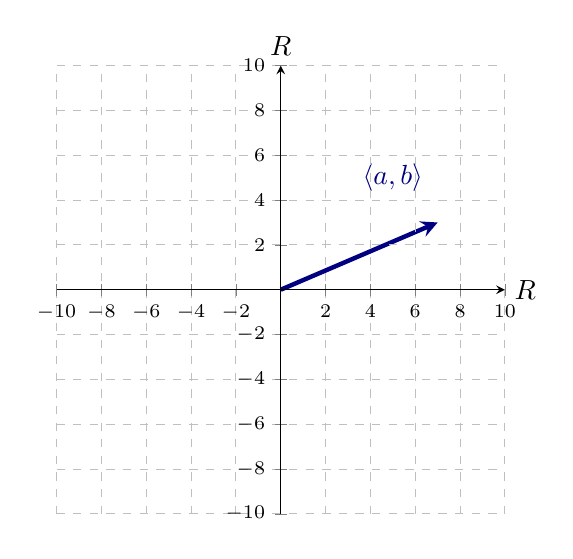
\begin{tikzpicture}
  \begin{axis}[
            domain=-10:10, ymax=10, xmax=10, ymin=-10, xmin=-10,
            axis lines =center, xlabel=$\mathbb{R}$, ylabel=$\mathbb{R}$, grid = major, grid style={dashed},
            unit vector ratio*=1 1 1,
            ytick={-10,-8,-6,-4,-2,2,4,6,8,10},
            xtick={-10,-8,-6,-4,-2,2,4,6,8,10},
            yticklabels={$-10$,$-8$,$-6$,$-4$,$-2$,$2$,$4$,$6$,$8$,$10$}, 
            xticklabels={$-10$,$-8$,$-6$,$-4$,$-2$,$2$,$4$,$6$,$8$,$10$},
            ticklabel style={font=\scriptsize},
            every axis y label/.style={at=(current axis.above origin),anchor=south},
            every axis x label/.style={at=(current axis.right of origin),anchor=west},
            axis on top
          ]


            \draw[penColor,ultra thick,->] (axis cs:0,0) -- (axis cs:7,3);
 

            \node at (axis cs:5,5) [penColor] {$\langle a, b \rangle$};





  \end{axis}
\end{tikzpicture}
\end{image}



Our vector notation $\langle a, b \rangle$ wraps together two components, which we could stretch out.

\[    \langle a, b \rangle = a \cdot \langle 1, 0 \rangle + b \cdot \langle 0, 1 \rangle            \]


\begin{notation} \textbf{\textcolor{blue!55!black}{Unit Component Vectors}}  \\

$\blacktriangleright$ $\langle 1, 0 \rangle$ is often written as $\hat{x}$ \\

$\blacktriangleright$ $\langle 0, 1 \rangle$ is often written as $\hat{y}$ \\

\end{notation}


These component vectors are the horizontal and vertical components of $\langle a, b \rangle$.


\[    \langle a, b \rangle = a \cdot \langle 1, 0 \rangle + b \cdot \langle 0, 1 \rangle  =  a \, \hat{x} + b \, \hat{y}         \]




\begin{image}
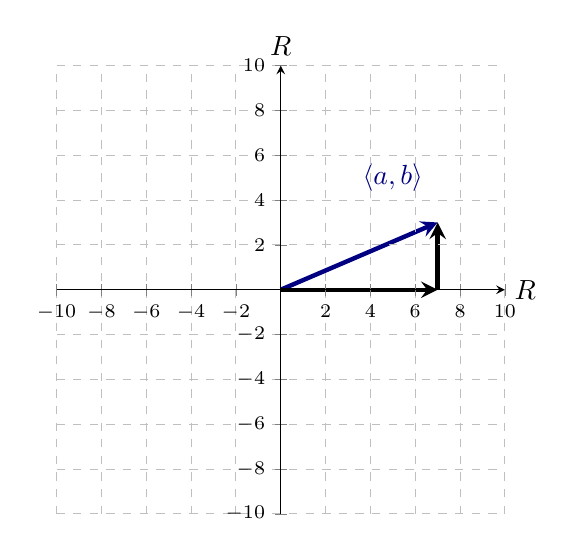
\begin{tikzpicture}
  \begin{axis}[
            domain=-10:10, ymax=10, xmax=10, ymin=-10, xmin=-10,
            axis lines =center, xlabel=$\mathbb{R}$, ylabel=$\mathbb{R}$, grid = major, grid style={dashed},
            unit vector ratio*=1 1 1,
            ytick={-10,-8,-6,-4,-2,2,4,6,8,10},
            xtick={-10,-8,-6,-4,-2,2,4,6,8,10},
            yticklabels={$-10$,$-8$,$-6$,$-4$,$-2$,$2$,$4$,$6$,$8$,$10$}, 
            xticklabels={$-10$,$-8$,$-6$,$-4$,$-2$,$2$,$4$,$6$,$8$,$10$},
            ticklabel style={font=\scriptsize},
            every axis y label/.style={at=(current axis.above origin),anchor=south},
            every axis x label/.style={at=(current axis.right of origin),anchor=west},
            axis on top
          ]


            \draw[penColor,ultra thick,->] (axis cs:0,0) -- (axis cs:7,3);
            \draw[black,ultra thick,->] (axis cs:0,0) -- (axis cs:7,0);
            \draw[black,ultra thick,->] (axis cs:7,0) -- (axis cs:7,3);
 

            \node at (axis cs:5,5) [penColor] {$\langle a, b \rangle$};





  \end{axis}
\end{tikzpicture}
\end{image}




\section*{Arithmetic Shorthand}



We have already noted that the real numbers are embedded in our plane as horizontal vectors.

$\blacktriangleright$  As algebraic shorthand notation, let's symbolize $a \cdot \langle 1, 0 \rangle = \langle a, 0 \rangle$ as $a$.  It is a horizontal vector and therefore represents a real number, so let's just represent it as we would a real number.



$\blacktriangleright$  As algebraic shorthand notation, the vector $ \langle 0, 1 \rangle $ is historically abbreviated as $i$.  \\




With these abbreviations, our 2-dimensional numbers now look like this


\begin{align*}
\langle a, b \rangle & = \langle a, 0 \rangle + \langle 0, b \rangle  \\
         & = \langle a, 0 \rangle + b \cdot \langle 0, 1 \rangle  \\
          & = a + b \, i
\end{align*}




Our 2-dimensional numbers have several representations.  Points and vectors are a geometric view, which will use extensively.


 $a + b \, i$, is our algebraic representation of the \textbf{Complex Numbers}. \\







\begin{definition}  \textbf{\textcolor{green!50!black}{Complex Numbers}}  \\


\[   \mathbb{C}  = \{  a + b \, i   \, | \, a, b \in \mathbb{R}             \}               \]


\end{definition}













The Complex Numbers are our algebraic view of our new 2-dimensional numbers.  In our story, the line between geometry and algebra is very blurry. It is almost like having double vision.  


\begin{itemize}
\item We have a geometric plane mapped out with points and coordinates.
\item We have a geometric plane in which we move about by vectors.
\item We have a 2-dimensional number system, where numbers are represented by points and vectors.
\item We have algebraic shorthand symbols where $i$ represents $\langle 0, 1 \rangle$.
\item We have our old real numbers, which are embedded in the new system as horizontal vectors or points on the horizontal axis. $1$ is represented by $\langle 1, 0 \rangle$ and can be written as $1 + 0 \, i$ or just $1$.
\end{itemize}





We hold all of these views on top of each other simultaneously and use the strength of each in our reasoning.





As noted before, multiplication by $i$ rotates counterclockwise $90^{\circ}$. What about twice?


\[  1 \cdot i \cdot i = -1    \]



If you rotate $1 = \langle 1, 0 \rangle$, $90^{\circ}$ counterclockwise, twice, then  you end up with $\langle 0,-1 \rangle = -1$





\[   i^2 = -1\]



\[   i = \sqrt{-1}   \]




Whoa!  We were looking for this number when studying the quadratic formula.  


\begin{center}
\textbf{\textcolor{red!80!black}{$i$ is the missing piece to the puzzle!}}
\end{center}








\textbf{\textcolor{purple!50!blue!90!black}{History}}


Mathematics has been a part of human thought for thousands of years.  Many people in many different countries have thought about mathematics over centuries.  And, unlike today, communication was not always easy.  Therefore, we have many groups of people inventing different notation and language for the same thing.  

We have to live with this history.

That means we have names and symbols for stuff that seems silly now, but it was serious business a couple of centuries ago.

For historical reasons the horizontal axis is called the \textbf{real axis} and the vertical axis is called the \textbf{imaginary axis}.  Complex numbers of the form $0 + a \, i$, like $i$, are called \textbf{imaginary numbers} - because a couple of centuries ago people thought this was all in our imagination.


A complex number, $a + b \, i$, has a real part, $Re(a + b \, i)= a$, and an imaginary part, $Im( a + b \, i)= b$.

That is the langugage we are stuck with.










\begin{example} Complex Numbers







\begin{image}
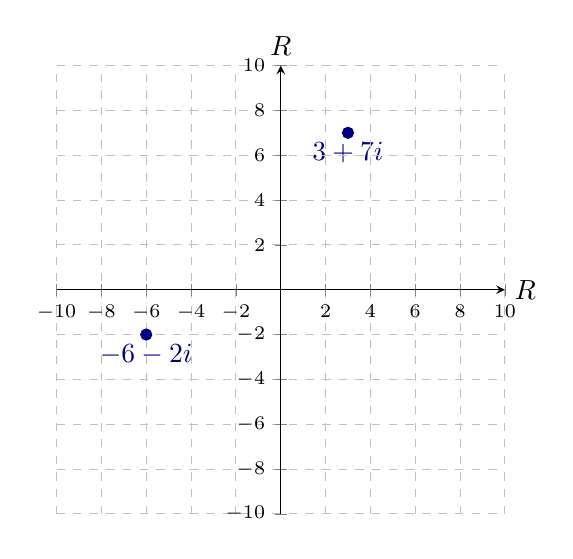
\begin{tikzpicture}
  \begin{axis}[
            domain=-10:10, ymax=10, xmax=10, ymin=-10, xmin=-10,
            axis lines =center, xlabel=$\mathbb{R}$, ylabel=$\mathbb{R}$, grid = major, grid style={dashed},
            unit vector ratio*=1 1 1,
            ytick={-10,-8,-6,-4,-2,2,4,6,8,10},
            xtick={-10,-8,-6,-4,-2,2,4,6,8,10},
            yticklabels={$-10$,$-8$,$-6$,$-4$,$-2$,$2$,$4$,$6$,$8$,$10$}, 
            xticklabels={$-10$,$-8$,$-6$,$-4$,$-2$,$2$,$4$,$6$,$8$,$10$},
            ticklabel style={font=\scriptsize},
            every axis y label/.style={at=(current axis.above origin),anchor=south},
            every axis x label/.style={at=(current axis.right of origin),anchor=west},
            axis on top
          ]


			\addplot[color=penColor,fill=penColor,only marks,mark=*] coordinates{(3,7)}; 
			\addplot[color=penColor,fill=penColor,only marks,mark=*] coordinates{(-6,-2)}; 
 

            \node at (axis cs:3,7) [penColor,anchor=north] {$3+7i$};
            \node at (axis cs:-6,-2) [penColor,anchor=north] {$-6-2i$};





  \end{axis}
\end{tikzpicture}
\end{image}




\begin{itemize}
\item $Re(3+7i) = 3$
\item $Im(3+7i) = 7$
\end{itemize}


\begin{itemize}
\item $Re(-6-2i) = -6$
\item $Im(-6-2i) = -2$
\end{itemize}


\end{example}











If we represented Complex Numbers with vectors, then each vector would have a \textbf{length}.  Inside our algebraic viewpoint, $a + b \, i$ doesn't have a length. It has a \textbf{modulus}.  The symbol for the modulus looks exactly like the absolute value symbol.

\begin{definition} \textbf{\textcolor{green!50!black}{Modulus}} \\
\[      |a + b \, i|    = \sqrt{a^2 + b^2}   \]
\end{definition}

The length of $\langle a, b \rangle$ equals the modulus of $a + b \, i$, both equal $\sqrt{a^2 + b^2}$













\begin{example} Unit Circle


We can now describe curves in the Cartesian plane via equations using complex numbers.

The unit circle is the collection of all points a distance of $1$ from the origin.  We can idenitfy these points via complex numbers.  The unit circle consists of the complex numbers whose modulus equals $1$

\[  |z| = 1  \]


\begin{image}
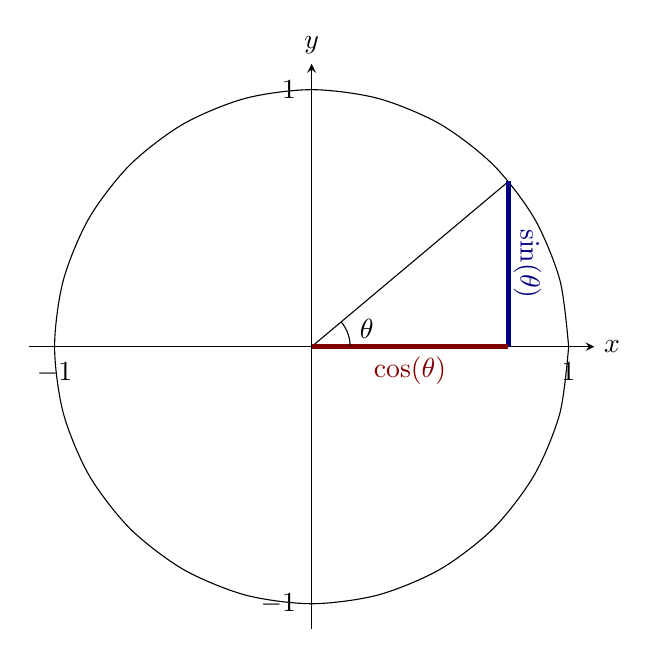
\begin{tikzpicture}
  \begin{axis}[
            xmin=-1.1,xmax=1.1,ymin=-1.1,ymax=1.1,
            axis lines=center,
            width=4in,
            xtick={-1,1},
            ytick={-1,1},
            clip=false,
            unit vector ratio*=1 1 1,
            xlabel=$x$, ylabel=$y$,
            every axis y label/.style={at=(current axis.above origin),anchor=south},
            every axis x label/.style={at=(current axis.right of origin),anchor=west},
          ]        
          \addplot [smooth, domain=(0:360)] ({cos(x)},{sin(x)}); %% unit circle

          \addplot [textColor] plot coordinates {(0,0) (.766,.643)}; %% 40 degrees

          \addplot [ultra thick,penColor] plot coordinates {(.766,0) (.766,.643)}; %% 40 degrees
          \addplot [ultra thick,penColor2] plot coordinates {(0,0) (.766,0)}; %% 40 degrees
          
          %\addplot [ultra thick,penColor3] plot coordinates {(1,0) (1,.839)}; %% 40 degrees          

          \addplot [textColor,smooth, domain=(0:40)] ({.15*cos(x)},{.15*sin(x)});
          %\addplot [very thick,penColor] plot coordinates {(0,0) (.766,.643)}; %% sector
          %\addplot [very thick,penColor] plot coordinates {(0,0) (1,0)}; %% sector
          %\addplot [very thick, penColor, smooth, domain=(0:40)] ({cos(x)},{sin(x)}); %% sector
          \node at (axis cs:.15,.07) [anchor=west] {$\theta$};
          \node[penColor, rotate=-90] at (axis cs:.84,.322) {$\sin(\theta)$};
          \node[penColor2] at (axis cs:.383,0) [anchor=north] {$\cos(\theta)$};
          %\node[penColor3, rotate=-90] at (axis cs:1.06,.322) {$\tan(\theta)$};
        \end{axis}
\end{tikzpicture}
\end{image}







On the unit circle, the coordinates of the points are $(\cos(\theta), \sin(\theta))$.  Therefore the real and  imaginary parts of complex numbers on the unit circle must also be $\cos(\theta)$ and $\sin(\theta)$.





The Unit Circle consists of all complex numbers of the form $\cos(\theta) + \sin(\theta) \, i$

\end{example}




















\begin{definition}  \textbf{\textcolor{green!50!black}{Complex Arithmetic}} \\



\begin{itemize}
\item $ (a + b \, i) + (c + d \, i) = (a+c) + (b+d) \, i$
\item $ (a + b \, i) - (c + d \, i) = (a-c) + (b-d) \, i$
\item $ (a + b \, i) \cdot (c + d \, i) = (ac-bd) + (ad+bc) \, i$
\end{itemize}


\end{definition}









\textbf{Note:} We still need to figure out division






\begin{question}


Compute   $(4 + 2 \, i) \cdot (-1 + i) = \answer{-6} + \answer{2} \, i$

\end{question}





\begin{question}


\begin{itemize}
\item Compute   $i^2 = i \cdot i = \answer{-1} + \answer{0} \, i$
\item Compute   $i^3 =  \answer{0} + \answer{-1} \, i$
\item Compute   $i^4 =  \answer{1} + \answer{0} \, i$
\item Compute   $i^5 =  \answer{0} + \answer{1} \, i$
\item Compute   $i^6 =  \answer{-1} + \answer{0} \, i$
\item Compute   $i^7 =  \answer{0} + \answer{-1} \, i$
\item Compute   $i^8 =  \answer{1} + \answer{0} \, i$
\end{itemize}

\end{question}


The calculations above demonstrate that $i = \sqrt{-1}$, which means that $i^2 = -1$.  It also means that $i^4 = 1$ and then we start all over.  The powers if $i$ are cyclic with a period of $4$.  Visually, on the unit circle, the powers of $i$ rotate around the unit circle in jumps of $90^{\circ} or \frac{\pi}{2}$ radians.

\begin{question}


$\sqrt{-9} = \sqrt{9} \cdot \sqrt{-1} =  \answer{3} \, i$

\end{question}

This presents some calculations, which, in previous courses, we would have avoided. And, for good reason:\\

\[  1 = \sqrt{1} = \sqrt{-1 \cdot -1} = \sqrt{-1} \cdot \sqrt{-1} = i \cdot i = -1   \]


The reason is that, in earlier courses, we simply declared that $\sqrt{number}$ is ALWAYS a positive number.  Now, we need to expand our calculational thinking. $\sqrt{1}$ could be $1$ or $-1$. \\

Usually, we do this by differentiating between radicals and fractional exponents.\\

\begin{itemize}
\item $\sqrt{r}$ still represents a positive real number if $r$ is a positive real number.
\item $\sqrt{-1} = i$ rather than $-i$.
\item $c^{\tfrac{1}{2}}$ will represent TWO numbers until someone specifies one of them.
\end{itemize}

That's where we'll begin.  It is not the complete story, but it will get us going.  More details coming up later.

















\begin{center}
\textbf{\textcolor{green!50!black}{ooooo-=-=-=-ooOoo-=-=-=-ooooo}} \\

more examples can be found by following this link\\ \link[More Examples of Complex Arithmetic]{https://ximera.osu.edu/csccmathematics/precalculus/precalculus/complexNumbers/examples/exampleList}

\end{center}




\end{document}
